%%%%%%%%%%%%%%%%%%%%%%%%%%%%%%%%%%%%%%%%%%%%%%%%%%%%%%%%%%%%%%%%%%%%%%%%%%%%%%%%%%%%%%%%%%%%
%%
%% Chapter 5 : Current progress
%%
%%      * Should describe the current state we are in the implementations, research, etc.
%%
%%%%%%%%%%%%%%%%%%%%%%%%%%%%%%%%%%%%%%%%%%%%%%%%%%%%%%%%%%%%%%%%%%%%%%%%%%%%%%%%%%%%%%%%%%%%

\chapter{Current progress}
\label{ch:current_progress}

%%%%%%%%%%%%%%%%%%%%%%%%%%%%%%%
%   Figures for chapter 5
%%%%%%%%%%%%%%%%%%%%%%%%%%%%%%%

\newcommand{\figProgressAgents}{
    \begin{figure}
        \centering
        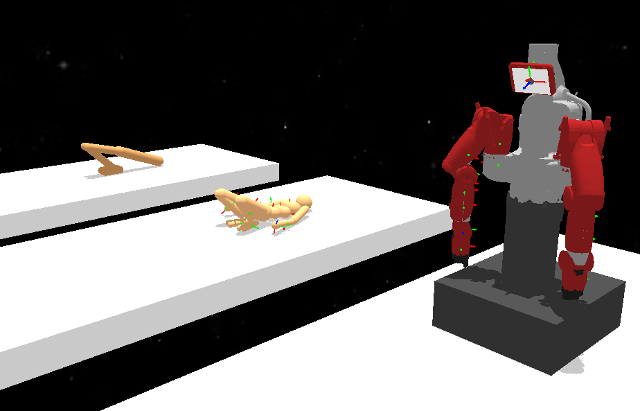
\includegraphics[width=0.9\textwidth]{./chapters/chapter_5/imgs/img_tysocmjc_agents.png}
        \caption{Current agent support. Currently the framework support mjcf
                 formats (from the mujoco engine)}
        \label{fig:ch5_progress_agents}
    \end{figure}
}

\newcommand{\figProgressSensors}{
    \begin{figure}
        \centering
        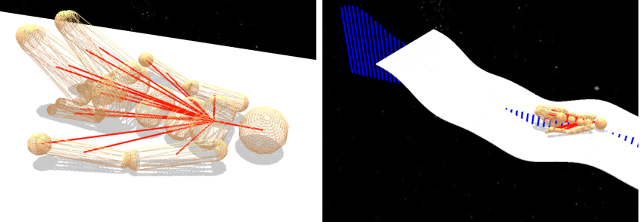
\includegraphics[width=0.9\textwidth]{./chapters/chapter_5/imgs/img_tysocmjc_sensors.png}
        \caption{Current sensor support. Currently the framework supports: 
                            a) intrinsic measurements (joint angles and velocities, body velocities and acceelrations, and relative positions).
                            b) extrinsic measurements (height fields taken from the terrain)}
        \label{fig:ch5_progress_sensors}
    \end{figure}
}

\newcommand{\figProgressTerrains}{
    \begin{figure}
        \centering
        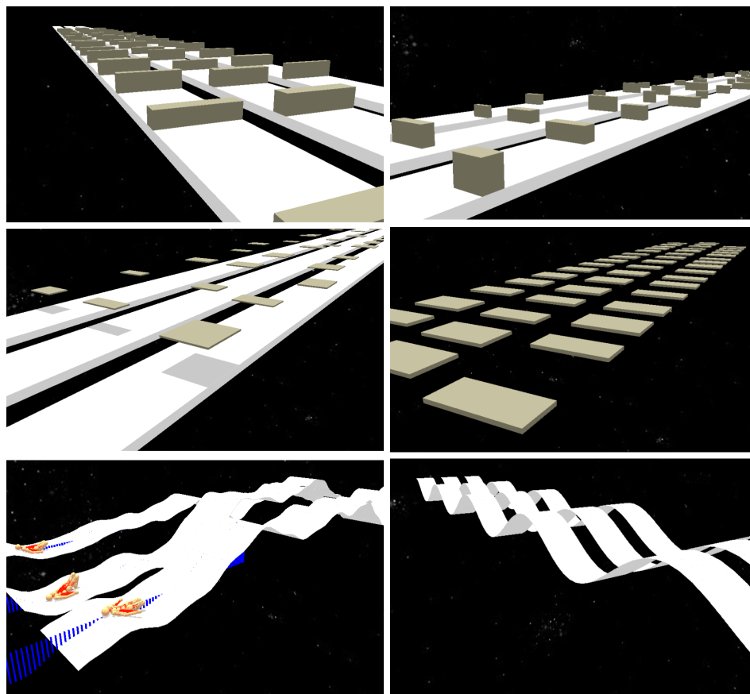
\includegraphics[width=0.9\textwidth]{./chapters/chapter_5/imgs/img_tysocmjc_terrains.png}
        \caption{Current terrain support. Currently the framework supports the
                 environments from \citeauthor{DeepmindEmergenceLocomotion}}
        \label{fig:ch5_progress_terrain}
    \end{figure}
}

\newcommand{\tableAgentFormatsSupport}{
    \begin{table}[]
        \centering
        \begin{tabular}{c|c|c|c|}
        \cline{2-4}
                                        & \cellcolor[HTML]{C0C0C0}{\color[HTML]{333333} mjcf} & \cellcolor[HTML]{C0C0C0}{\color[HTML]{333333} urdf} & \cellcolor[HTML]{C0C0C0}{\color[HTML]{333333} rlsim} \\ \hline
        \multicolumn{1}{|c|}{Completed} & x                                                   & x                                                   &                                                      \\ \hline
        \multicolumn{1}{|c|}{Tested}    & x                                                   &                                                     &                                                      \\ \hline
        \end{tabular}
        \caption{Current agent formats supported in the framework}
        \label{tab:ch5_table_supported_agent_formats}
    \end{table}
}

\newcommand{\tableBackendsSupport}{
    \begin{table}[]
        \centering
        \begin{tabular}{c|c|c|}
        \cline{2-3}
                                        & \cellcolor[HTML]{C0C0C0}{\color[HTML]{333333} MuJoCo} & \cellcolor[HTML]{C0C0C0}{\color[HTML]{333333} Bullet} \\ \hline
        \multicolumn{1}{|c|}{Completed} & x                                                     &                                                       \\ \hline
        \multicolumn{1}{|c|}{Tested}    & x                                                     &                                                       \\ \hline
        \end{tabular}
        \caption{Current backends supported in the framework}
        \label{tab:ch5_table_supported_backends}
    \end{table}
}

In this chapter we discuss the current progress of the proposed framework. 
The implementation is still not in version 0.1, which should be the first 
fully functional version to be released according to the features proposed 
in the previous chapter. Nevertheless, the core functionality, which is related
to the abstract representations (section ~\ref{subsec:ch4_core_functionality}),
is working and almost completed. There is also a working implementation for
MuJoCo, one of the two backends that we will support. All the implementations 
are available in github, in the following repositories:

\begin{itemize}
    \item \textbf{Core functionality}: the repository that serves as the
          core dependency for the framework. It can be found \href{https://github.com/wpumacay/tysocCore}{here}
          \footnote{https://github.com/wpumacay/tysocCore}.
    \item \textbf{MuJoCo implementation}: the repository with the
          adapter code for MuJoCo as the specific backend. It can be found
          \href{https://github.com/wpumacay/tysocMjc}{here} \footnote{https://github.com/wpumacay/tysocMjc}.
\end{itemize}

\section{Core functionality}

As previously mentioned we already have a working implementation of the core
functionality supporting part of the proposed agent formats, and the appropriate
abstractions for the terrain and sensors. This functionality is decoupled of the 
specific backend we used for instantiating the simulation. The key components currently 
available are the following:

\begin{itemize}
    \item \textbf{Agent core functionality}: We implemented the core kinematic 
            tree (explained previously in Figure ~\ref{fig:ch4_core_agent_functionality}), 
            and made sure that this implementation was decoupled from the backend by
            following the bridge approach mentioned in section ~\ref{fig:ch4_bridge_pattern}.
            We currently have support for the \textbf{mjcf} and \textbf{urdf} agent 
            formats. We have also support for three agents from the proposed agents list:
            walker and humanoid from Controlsuite, and laikago from PyBullet. These
            are shown in the Figure below.

            \figSupportedAgents

    \item \textbf{Terrain core functionality}: We implemented the abstract terrain
           functionality (explained previously in Figure ~\ref{fig:ch4_core_terrain_functionality}),
           and also two simple procedural terrain generators: one for forward running
           tasks with terrain generated using boxes as primitives, similar to the
           terrain used in \cite{DeepmindEmergenceLocomotion}, and the other also
           for forward running tasks using variable height terrain generated from a
           profile, connected by boxes as primitives.

           \figSupportedTerrain
    \newpage
    \item \textbf{Sensors core functionality}: We implemented the core sensors
          functionality and made sure that this implementation was decoupled from
          the backend, following the bridge approach mentioned in section ~\ref{fig:ch4_bridge_pattern}.
          The sensors currently supported by the framework consist of intrinsic
          measurements from joints and bodies, and extrinsic readings from the
          terrain using heightfields.

          \figSupportedSensors

\end{itemize}

%% @TODO: talk about the visualizer, and the two implemented options.
%% @TODO: make a table to list done and todos in this feature

%% @TODO: talk about the backends supported so far
%% @TODO: make a table to list done and todos in this feature

\section{Simulation features}

As previously mentioned, the current backend that the framework supports is the
MuJoCo physics engine. The implementation was made with the bridge approach shown
in Figure ~\ref{fig:ch4_bridge_pattern}, and extra care was taken to ensure not
to couple backend specific features in the core framework. 

Although this section will look as a repetition of the previous section, recall
that this functionality is specific for a specific backend. Currently we just have
one backend, but in the next few months we expect to have the full implementation
for all proposed backends, and some slight details will appear for each one. The 
current support for the MuJoCo backend contains the following:

\begin{itemize}
    \item \textbf{Agent support}: This implementation allows the instantiation of 
          various agents using the MuJoCo backend. There is also support for setting 
          control commands through the C/C++ low-level API, which allows to do 
          experiments similar to current benchmarks that also use MuJoCo. For a reference 
          video visit \href{https://youtu.be/5zv5SK0o92I}{this} link \footnote{https://youtu.be/5zv5SK0o92I}.

    \item \textbf{Terrain support}: The framework currently allows the instantiation 
          of the two core terrain generators using the MuJoCo backend. For a reference 
          video visit \href{https://youtu.be/xWdNFGlhlOA}{this} link \footnote{https://youtu.be/xWdNFGlhlOA}.

    \item \textbf{Sensors support}: The implementation allows the user to take 
          measurements from the instantiated agents in the mujoco backend. Both
          types sensors mentioned earlier are supported. For reference 
          videos visit \href{https://youtu.be/-EJMER5AGRQ}{this} \footnote{https://youtu.be/-EJMER5AGRQ} and 
          \href{https://youtu.be/c0R81VBZ72o}{this} \footnote{https://youtu.be/c0R81VBZ72o} 
          links for extrinsic and intrinsic measurements respectively.

    \item \textbf{Instantiation support}: The current approach for instantiating
          with the MuJoCo backend consists of making use of XML injection. The
          current MuJoCo API only allows to create a simulation through an XML
          file that is compiled at initialization, and unlike other backends there
          is currently no runtime creation API. 

          In order to achieve the desired functionality we inject all the simulation
          resources into an XML that MuJoCo can then use to instantiate the scene,
          and making heavy use of object pools to reuse the resources that are
          defined in the XML file. A sample generated XML with all resources can
          be found \href{https://github.com/wpumacay/tysocMjc/blob/master/res/xml/workspace.xml}{here}
          \footnote{https://github.com/wpumacay/tysocMjc/blob/master/res/xml/workspace.xml}
          (which is a big XML file), and a sample model for an agent can be found
          \href{https://github.com/wpumacay/tysocMjc/blob/master/res/templates/mjcf/walker.xml}{here}
          \footnote{https://github.com/wpumacay/tysocMjc/blob/master/res/templates/mjcf/walker.xml}.

          The approach of using core functionality separated from backend specific
          functionality helps a lot in this situation because we do not have to
          couple the specific instantiation mechanisms (like in MuJoCo) to other
          mechanisms (like in Bullet and PhysX), and in the case that MuJoCo launches
          a release in the future with runtime creation support we can easily change
          the adapter code once and all other backend options will not need to be
          changed at all.

    \item \textbf{Visualizer support}: In order to test the correctness of the
          implementation we need an interactive mechanism to view the simulation.
          The framework is designed to be renderer agnostic, and currently we support
          two types of renderers: a custom redenrer using OpenGL, and the provided
          MuJoCo renderer. This two options are shown in Figure ~\ref{fig:ch5_current_supported_visualizers}.

          We plan to implement also a variation of our custom renderer based on
          EGL, which allows to create a rendering context without an active windowing
          system, like the case of running experiments in the cloud (Amazon Web Services,
          Google Cloud, etc.). This feature will be important in the case of running
          experiments in a cluster, which is very likely because DeepRL algorithms
          tend to need lots of samples, and distributed setups is usually a good
          option to speed up experimentation.

          \newpage
          \figSupportedVisualizers

\end{itemize}

\section{Summary}

In this chapter we presented various details of our current implementation and
the features currently available. Some key aspects discussed in this chapter are:

\begin{itemize}
    \item The current implementation already supports the features proposed, namely
          agents, terrain and sensors creation. All these features were implemented
          by decoupling the implementation from any backend specific, which will help 
          to support various physics and rendering backends without much change.

    \item The current implementation supports one physics backend (MuJoCo),
          having support for the core features (agents, terrain and sensors) and
          already allowing simulation and experiments through a C/C++ API.
          We also have support for two rendering backends: a custom rendering backend,
          and the rendering backend shipped along the MuJoCo physics engine 
          (see Figure ~\ref{fig:ch5_current_supported_visualizers}).

    \item This implementation also has support for some of the agents that were
          proposed for the evaluation experiments (see Figure ~\ref{fig:ch5_current_supported_agents}).
          We also reproduced (as a proof of concept) the terrain from \cite{DeepmindEmergenceLocomotion} 
          by implementing the appropiate terrain generators (see Figure ~\ref{fig:ch5_current_supported_terrain}),
          and some sensors used in various related works (see Figure ~\ref{fig:ch5_current_supported_sensors}).
\end{itemize}